\section{Удлинение пути}
\textbf{Вопрос.} На сколько бетатрон удлиняет путь, если полость включена и синхротрон уже идёт?

Две частицы в одном кольце: одна без бетатронной амплитуды, другая с $A=20$~мм. Рисунок --- разность их лишних длин, не прогон с $V=0$. Формула $\Lambda=-(2\pi/C)J\xi$.

\begin{figure}[H]\centering
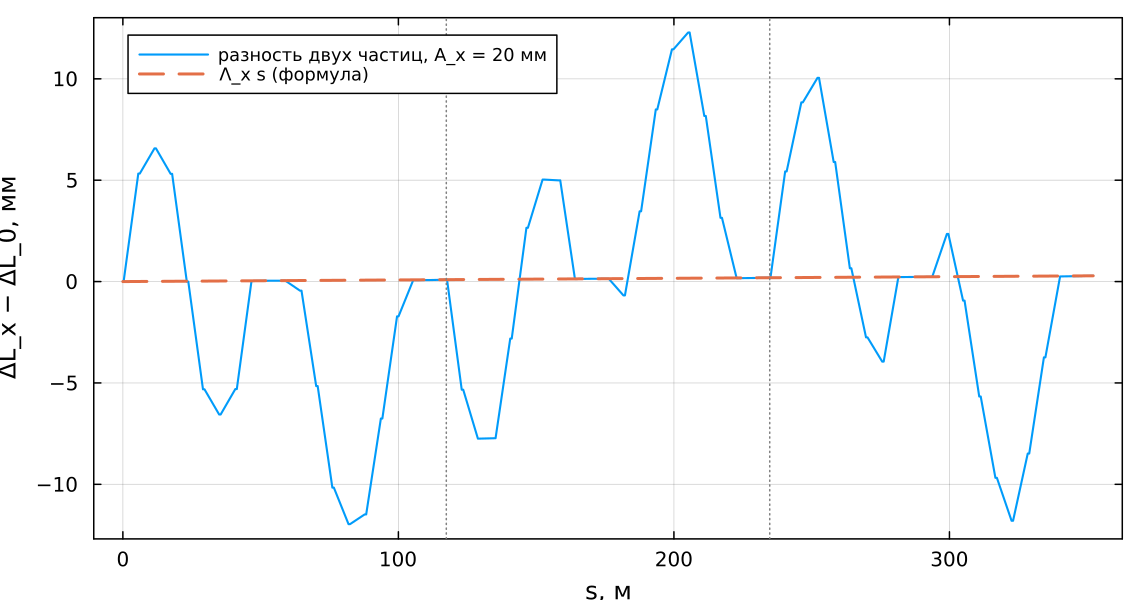
\includegraphics[width=0.92\textwidth]{figs/fig_05_path_x.png}
\caption{Плоскость $x$. Наклон формулы $\Lambda_x=\vLamX$.}
\end{figure}

\begin{figure}[H]\centering
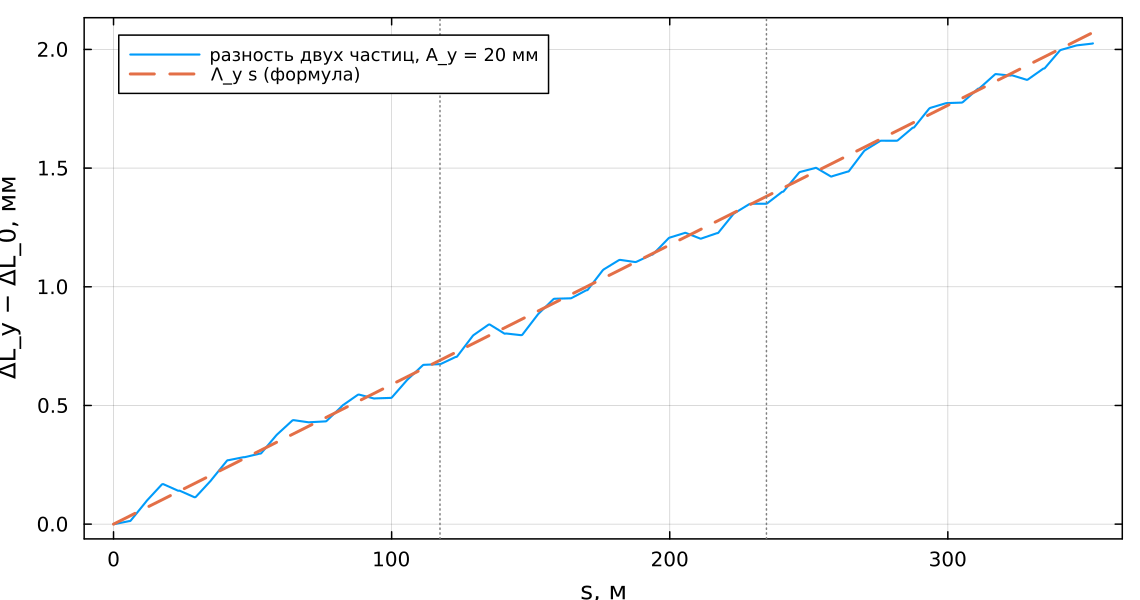
\includegraphics[width=0.92\textwidth]{figs/fig_05_path_y.png}
\caption{Плоскость $y$. Наклон формулы $\Lambda_y=\vLamY$.}
\end{figure}

\begin{figure}[H]\centering
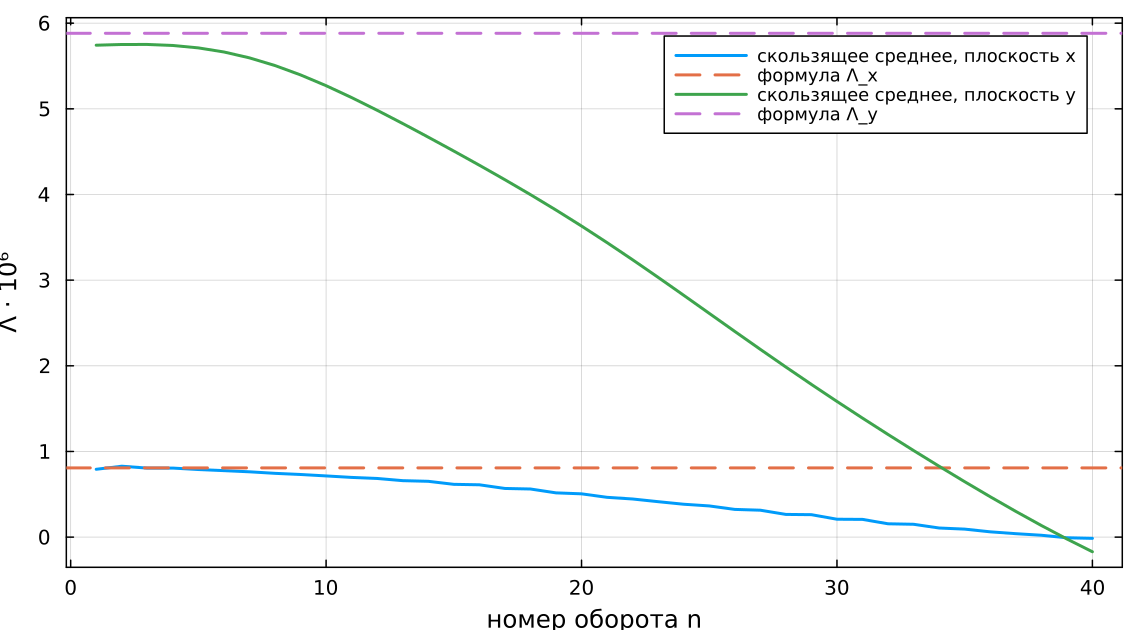
\includegraphics[width=0.92\textwidth]{figs/fig_05_path_mean.png}
\caption{Пооборотная разность за первые $\vNfpath$ оборотов, пока синхротронные фазы ещё не разбежались. Наклон $\Delta L(s)$ за три оборота: $x$ $\vLamXtr$ (формула $\vLamX$, разница $\vDiffLamX$), $y$ $\vLamYtr$ (формула $\vLamY$, разница $\vDiffLamY$).}
\end{figure}

\textbf{Вывод.} В плоскости $y$ наклон за три оборота совпадает с формулой (разница $\vDiffLamY$). В плоскости $x$ $\Lambda$ меньше, за три оборота его ещё закрывает бетатронное колебание длины --- смотреть тренд на рисунке, не линейную подгонку. На многих оборотах синхротронные фазы двух частиц разбегаются.
